\documentclass[letterpaper]{article}

\usepackage[mmddyy]{datetime}
\usepackage[margin=1.25in]{geometry}
\usepackage{fancyhdr}
\usepackage{amsmath}
\usepackage{amssymb}
\usepackage{graphicx}

\usepackage{listings}
\usepackage{color}

\definecolor{codeblue}{rgb}{0.2039, 0.5961, 0.8588}
\definecolor{codegreen}{rgb}{ 0.3451, 0.8392, 0.5529}
\definecolor{codedark}{rgb}{  0.2039, 0.2863, 0.3686}
\definecolor{backcolour}{rgb}{0.9176, 0.9255, 0.9333}
\definecolor{codepink}{rgb}{0.9804, 0.5490, 0.7725}

\lstdefinestyle{mystyle}{
    backgroundcolor=\color{backcolour},
    commentstyle=\color{codegreen},
    keywordstyle=\color{codeblue},
    numberstyle=\tiny\color{codedark},
    stringstyle=\color{codepink},
    basicstyle=\footnotesize,
    basicstyle=\footnotesize\fontfamily{\ttdefault}\selectfont,
    breakatwhitespace=false,
    breaklines=true,
    captionpos=b,
    keepspaces=true,
    numbers=left,
    numbersep=5pt,
    showspaces=false,
    showstringspaces=false,
    showtabs=false,
    tabsize=2
}

\lstset{style=mystyle}

\pagestyle{fancy}
\fancyhf{}
\rhead{Cort Breuer}
\chead{\today}
\lhead{ENGRD 2700}
\rfoot{\thepage}

\begin{document}

\vspace*{6pt}

\noindent \textbf{\huge{Problem Set 5}}

\bigskip

\section*{Question 1}

Joint density function given by $f_{X, Y}(x, y)=\left\{\begin{array}{ll}{k(2 y+x y)} & {\text { if } 0 \leq x \leq 1 \text { and } x \leq y \leq 1} \\ {0} & {\text { otherwise. }}\end{array}\right$

\subsection*{Part A}

$$\int \int f_{X,Y} (x, y) dx dy = 1$$

$$\int_0^1 \int_x^1 k(2y+xy) dy dx + \int \int 0 dx dy = 1$$


$$\int_0^1 \int_x^1 [ 2ky + kxy ] dy dx = 1$$

$$\int_0^1 [ ky^2 + \frac{1}{2} kxy^2 ] \Big|_x^1 dx = 1$$

$$\int_0^1 [ k - kx^2 + \frac{1}{2} kx - \frac{1}{2} kx^3] dx = 1$$

$$[ kx - \frac{1}{3} kx^3 + \frac{1}{4} kx^2 - \frac{1}{8} kx^4 ] \Big|_0^1 = 1$$

$$k[1 - 0] - \frac{1}{3}[k - 0] + \frac{1}{4}[k - 0] - \frac{1}{8}[k - 0] = 1$$

$$k - \frac{k}{3} + \frac{k}{4} - \frac{k}{8} = 1$$

$$k \frac{19}{24}= 1$$

$$k = \frac{24}{19}$$

\subsection*{Part B}

$$\text{Marginal PDF of } X \ f_X(x) = \int f_{X, Y}(x, y) dy$$

$$f_X(x) = \int_0^1 k(2y + xy) dy = k(y + \frac{1}{2} xy^2) \Big|_0^1$$

$$f_X(x) = k \Big[ (1 + \frac{1}{2} x) - (0 + \frac{1}{2} 0) \Big] = \frac{24}{19} [1 + \frac{1}{2} x]$$

$$f_X(x) = \frac{24}{19} + \frac{12}{19} x$$

$$\text{Marginal PDF of } X \ f_X(x) = \begin{cases} \frac{24}{19} + \frac{12}{19} x & 0 \leq x \leq 1 \\ 0 & \text{otherwise} \end{cases}$$

\subsection*{Part C}

$$f_{X|Y} (x|y) = \frac{f_{X,Y}(x,y)}{f_Y(y)}$$

$$f_Y(y) = \int f_{X, Y}(x, y) dx = \int_0^y k(2y + xy) dx$$

$$f_Y(y) = k(2yx + \frac{1}{2} x^2y) \Big|_0^y = \frac{24}{19} (2y^2 + \frac{1}{2} y^3)$$

$$f_{X|Y} (x|y) = \frac{\frac{24}{19}(2y + xy)}{\frac{24}{19} (2y^2 + \frac{1}{2} y^3)} = \frac{2 + x}{2y + \frac{1}{2} y^2)}$$

$$f_{X|Y} (x|\frac{1}{4}) = \frac{2 + x}{\frac{1}{2} + \frac{1}{32}} = \frac{2 + x}{\frac{17}{32}} = \frac{64 + 32x}{17}$$

$$f_{X|Y} = \begin{cases} \frac{64 + 32x}{17} & 0 \leq x \leq \frac{1}{4} \\ 0 & \text{otherwise} \end{cases}$$

\section*{Question 2}

\subsection*{Part A}

\subsection*{Part B}

\subsection*{Part C}

\subsection*{Part D}

\subsection*{Part E}

\section*{Question 3}

\subsection*{Part A}

\subsection*{Part B}

\subsection*{Part C}

\section*{Question 4}

$$\text{Joint PDF given by } f_{X|Y}(x, y) = \begin{cases} 2ye^{-y(2+x)} & x, y \geq 0 \\ 0  & \text{otherwise} \end{cases}$$

$$f_{X|Y}(x|y) = \frac{f_{X,Y}(x, y)}{f_Y(y)}$$

$$f_Y(y) = \int_0^{\infty} 2ye^{-y(2+x)} dx = -2 \int_0^{\infty} e^u dx \text{ with } u = -y(2+x)$$

$$f_Y(y) = -2 e^u \Big|_0^{\infty} = -2 e^{-y(2+x)} \Big|_0^{\infty}$$

$$f_Y(y) = -2 e^{-y(2+ \infty)} + 2 e^{-y(2+0)} = 2 e^{-2y}$$

$$f_{X|Y}(x|y) = \frac{f_{X,Y}(x, y)}{f_Y(y)} = \frac{2ye^{-y(2+x)}}{2 e^{-2y}}$$

$$f_{X|Y}(x|y) = \frac{y e^{-2y} e^{-yx}}{e^{-2y}} = y e^{-yx}$$

$$f_{X|Y}(x|y) = \begin{cases} y e^{-yx} & x, y \geq 0 \\ 0 & \text{otherwise} \end{cases}$$

\section*{Question 5}

\begin{lstlisting}[language=R]
    Bwages <- read_csv("Bwages.csv")
\end{lstlisting}

\subsection*{Part A}

\begin{lstlisting}[language=R]
    ggplot(data = Bwages) + geom_histogram(mapping = aes(x = wage), binwidth = 3) + xlab("Wages") + ylab("Count")
\end{lstlisting}

\begin{center}
    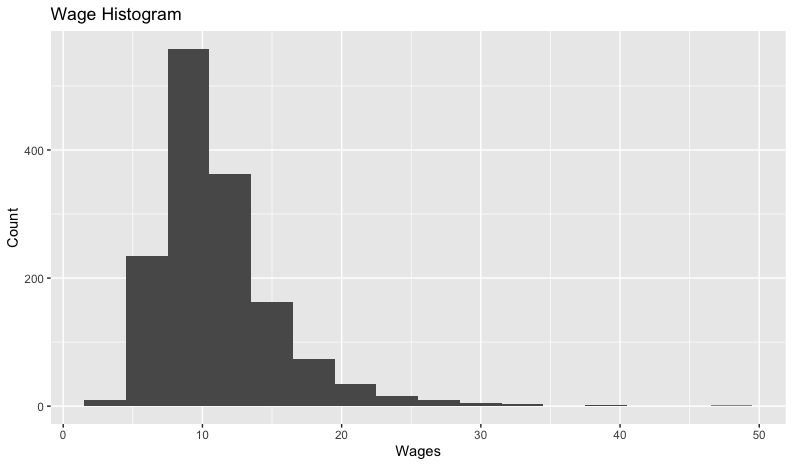
\includegraphics[width=6in]{wageHistogram.png}
\end{center}

\subsection*{Part B}

\subsection*{Part C}

\subsection*{Part D}

\subsection*{Part E}

\end{document}
